\documentclass[12pt,a4paper]{article}
\usepackage[utf8]{vietnam}
\usepackage{amsmath,amssymb}
\usepackage{tabularx}
\usepackage{tikz}
\usetikzlibrary{calc,angles,quotes,arrows.meta,patterns}
\usepackage{xcolor}
\usepackage{enumitem}
\usepackage{fancyhdr}
\usepackage{graphicx}
\usepackage[top=0.9cm, bottom=0.9cm, left=1.2cm, right=1.2cm]{geometry}
\usepackage[loigiai]{ex_test}
\SAOPTN{widthSA=3.2,heightSA=0.62}

\setlength{\headheight}{15pt}
\setlength{\parskip}{0pt}

\pagestyle{fancy}
\fancyhf{}
\rhead{\textit{Môn Toán 8 -- Hướng dẫn giải Đề số 08}}
\lhead{\textit{Bộ đề ôn tập Giữa học kì I}}
\cfoot{\thepage}

\begin{document}

\begin{center}
  \textbf{\Large HƯỚNG DẪN GIẢI CHI TIẾT VÀ BẢNG ĐÁP ÁN}\\
  \textbf{\large ĐỀ ÔN TẬP GIỮA HỌC KỲ I -- ĐỀ SỐ 08}\\
  \textit{Môn: Toán 8 -- Năm học 2026 -- 2027}
\end{center}
\vspace{2mm}

% --- BẢNG ĐÁP ÁN TRẮC NGHIỆM TÓM TẮT ---
\noindent\textbf{\large A. BẢNG ĐÁP ÁN TRẮC NGHIỆM TỔNG HỢP}
\vspace{1mm}

\noindent\textbf{1. Phần I (Mỗi câu trả lời đúng được 0,25 điểm):}
\begin{center}
\begin{tabular}{|c|c|c|c|c|c|c|c|c|c|c|c|c|}
\hline
\textbf{Câu} & \textbf{1} & \textbf{2} & \textbf{3} & \textbf{4} & \textbf{5} & \textbf{6} & \textbf{7} & \textbf{8} & \textbf{9} & \textbf{10} & \textbf{11} & \textbf{12} \\
\hline
\textbf{Đ/A} & \textbf{B} & \textbf{D} & \textbf{B} & \textbf{B} & \textbf{D} & \textbf{C} & \textbf{B} & \textbf{C} & \textbf{A} & \textbf{B} & \textbf{D} & \textbf{C} \\
\hline
\end{tabular}
\end{center}
\vspace{0.5mm}

\noindent\textbf{2. Phần II (Đúng 1 ý: 0,1đ; 2 ý: 0,25đ; 3 ý: 0,5đ; 4 ý: 1,0đ):}
\begin{center}
\begin{tabular}{|c|c|c|c|c||c|c|c|c|c|}
\hline
\textbf{Câu} & \textbf{a)} & \textbf{b)} & \textbf{c)} & \textbf{d)} & \textbf{Câu} & \textbf{a)} & \textbf{b)} & \textbf{c)} & \textbf{d)} \\
\hline
\textbf{Câu 1} & \textbf{Đ} & \textbf{Đ} & \textbf{Đ} & \textbf{S} & \textbf{Câu 2} & \textbf{Đ} & \textbf{Đ} & \textbf{S} & \textbf{Đ} \\
\hline
\end{tabular}
\end{center}
\vspace{0.5mm}

\noindent\textbf{3. Phần III (Mỗi câu trả lời đúng được 1,0 điểm):}
\begin{center}
\begin{tabular}{|c|c|c|}
\hline
\textbf{Câu} & \textbf{Câu 1} & \textbf{Câu 2} \\
\hline
\textbf{Đáp án} & $\mathbf{x = -4 \text{ hoặc } x = 6}$ & $\mathbf{5\text{ cm}}$ \\
\hline
\end{tabular}
\end{center}
\vspace{1.5mm}

% --- B. LỜI GIẢI CHI TIẾT ---
\noindent\textbf{\large B. LỜI GIẢI CHI TIẾT CÁC CÂU HỎI}
\vspace{1mm}
\begin{ex}
Giá trị của biểu thức $A = x^2 + 2y - 1$ tại $x = 1$ và $y = -1$ là:
\choice
{$-1$}
{\True $-2$}
{$1$}
{$2$}
\loigiai{
Thay $x = 1$ và $y = -1$ vào biểu thức $A$: $A = 1^2 + 2(-1) - 1 = 1 - 2 - 1 = -2$.
}
\end{ex}

\begin{ex}
Trong các đơn thức sau, đơn thức nào đồng dạng với đơn thức $5x^2y$?
\choice
{$5xy$}
{$4xy^2$}
{$7a^2b$}
{\True $-3x^2y$}
\loigiai{
Hai đơn thức đồng dạng có hệ số khác 0 và có cùng phần biến. Đơn thức $-3x^2y$ có phần biến là $x^2y$, trùng với phần biến của $5x^2y$.
}
\end{ex}

\begin{ex}
Kết quả của phép nhân $(a + 2)(a - 2)$ bằng:
\choice
{$a^2 + 4$}
{\True $a^2 - 4$}
{$a^2 - 2$}
{$a^2 - 1$}
\loigiai{
Áp dụng hằng đẳng thức hiệu hai bình phương: $(a + 2)(a - 2) = a^2 - 2^2 = a^2 - 4$.
}
\end{ex}

\begin{ex}
Giá trị của đa thức $-x^3y^2 + 2x$ tại $x = -1; y = 0$ là:
\choice
{$2$}
{\True $-2$}
{$-1$}
{$1$}
\loigiai{
Thay $x = -1$ và $y = 0$ vào đa thức: $-(-1)^3 \cdot 0^2 + 2(-1) = 0 - 2 = -2$.
}
\end{ex}

\begin{ex}
Biểu thức $(2x - y)^2$ có biểu thức khai triển là:
\choice
{$x^2 + 2xy + 2y^2$}
{$x^2 - 2xy + 2y^2$}
{$x^2 + 4xy + 4y^2$}
{\True $4x^2 - 4xy + y^2$}
\loigiai{
Áp dụng hằng đẳng thức bình phương của một hiệu: $(2x - y)^2 = (2x)^2 - 2 \cdot 2x \cdot y + y^2 = 4x^2 - 4xy + y^2$.
}
\end{ex}

\begin{ex}
Đơn thức nào sau đây đồng dạng với đơn thức $-3x^2y$?
\choice
{$\dfrac{1}{2}xy$}
{$3x^2yz$}
{\True $-2x^2y$}
{$-3x^2z$}
\loigiai{
Đơn thức $-2x^2y$ có cùng phần biến $x^2y$ với đơn thức $-3x^2y$ nên đồng dạng.
}
\end{ex}

\begin{ex}
Tích $(2x - 3)(2x + 3)$ có kết quả bằng:
\choice
{$4x^2 + 12x + 9$}
{\True $4x^2 - 9$}
{$2x - 3$}
{$4x - 9$}
\loigiai{
Áp dụng hằng đẳng thức hiệu hai bình phương: $(2x - 3)(2x + 3) = (2x)^2 - 3^2 = 4x^2 - 9$.
}
\end{ex}

\begin{ex}
Các góc của một tứ giác có thể là:
\choice
{Bốn góc nhọn}
{Bốn góc tù}
{\True Bốn góc vuông}
{Một góc vuông, ba góc nhọn}
\loigiai{
Tổng bốn góc của tứ giác luôn bằng $360^\circ$. Nếu tứ giác có 4 góc vuông thì tổng số đo là $90^\circ \cdot 4 = 360^\circ$ (thỏa mãn).
}
\end{ex}

\begin{ex}
Hình chữ nhật có hai đường chéo như thế nào?
\choice
{\True Bằng nhau và cắt nhau tại trung điểm mỗi đường}
{Bằng nhau}
{Cắt nhau tại trung điểm mỗi đường}
{Vuông góc với nhau}
\loigiai{
Theo tính chất hình chữ nhật, hai đường chéo bằng nhau và cắt nhau tại trung điểm của mỗi đường.
}
\end{ex}

\begin{ex}
Cho tam giác $ABC$ vuông tại $A$ như hình vẽ bên. Tính $x$:
\begin{center}
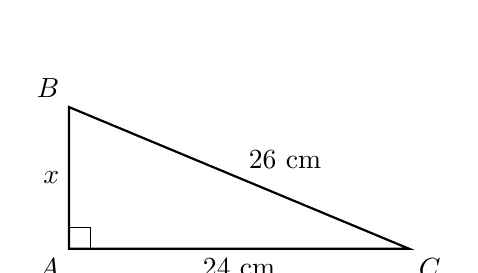
\begin{tikzpicture}[scale=0.18, >=stealth]
  \coordinate (A) at (0,0);
  \coordinate (C) at (24,0);
  \coordinate (B) at (0,10);
  \draw[thick] (A)--(C)--(B)--cycle;
  \draw (1.5,0) |- (0,1.5);
  \fill (A) circle (1.5pt) node[below left] {$A$};
  \fill (B) circle (1.5pt) node[above left] {$B$};
  \fill (C) circle (1.5pt) node[below right] {$C$};
  \node[left] at ($(A)!0.5!(B)$) {$x$};
  \node[below] at ($(A)!0.5!(C)$) {$24\text{ cm}$};
  \node[above right] at ($(B)!0.5!(C)$) {$26\text{ cm}$};
\end{tikzpicture}
\end{center}
\choice
{$x = 13\text{ cm}$}
{\True $x = 10\text{ cm}$}
{$x = 20\text{ cm}$}
{$x = 2\text{ cm}$}
\loigiai{
Áp dụng định lý Pythagore trong tam giác vuông $ABC$: $AB^2 + AC^2 = BC^2 \Rightarrow x^2 + 24^2 = 26^2 \Rightarrow x^2 = 676 - 576 = 100 \Rightarrow x = 10\text{ cm}$.
}
\end{ex}

\begin{ex}
Tam giác nào là tam giác vuông trong các tam giác có độ dài ba cạnh sau?
\choice
{$10\text{ m}; 13\text{ m}; 15\text{ m}$}
{$7\text{ mm}; 8\text{ mm}; 10\text{ mm}$}
{$6\text{ dm}; 7\text{ dm}; 9\text{ dm}$}
{\True $9\text{ cm}; 12\text{ cm}; 15\text{ cm}$}
\loigiai{
Ta có: $15^2 = 225$ và $9^2 + 12^2 = 81 + 144 = 225$. Vì $9^2 + 12^2 = 15^2$ nên theo định lý Pythagore đảo, đây là tam giác vuông.
}
\end{ex}

\begin{ex}
Cho hình chóp tứ giác đều có cạnh đáy bằng $10\text{ cm}$, chiều cao bằng $9\text{ cm}$. Thể tích của hình chóp tứ giác đều là:
\choice
{$30\text{ cm}^3$}
{$45\text{ cm}^3$}
{\True $300\text{ cm}^3$}
{$450\text{ cm}^3$}
\loigiai{
Diện tích đáy: $S = 10 \cdot 10 = 100\text{ cm}^2$. Thể tích: $V = \dfrac{1}{3} S \cdot h = \dfrac{1}{3} \cdot 100 \cdot 9 = 300\text{ cm}^3$.
}
\end{ex}


\setcounter{ex}{0}
\noindent\textbf{\large PHẦN II. CÂU TRẮC NGHIỆM ĐÚNG SAI}
\vspace{1mm}
\begin{ex}
Cho hai biểu thức $A = (x - 2)^2 - (x - 1)(x + 3)$ và $B = x^3 - 6x^2y + 12xy^2 - 8y^3$. Xét tính đúng sai của các mệnh đề sau:
\choiceTF
{\True Khai triển hằng đẳng thức $(x - 2)^2$ ta được $x^2 - 4x + 4$}
{\True Kết quả rút gọn của biểu thức $A$ là $-6x + 7$}
{\True Viết đa thức $B$ dưới dạng lập phương của một hiệu ta được $(x - 2y)^3$}
{Tại $x = 1$, giá trị của biểu thức $A$ bằng $-1$}
\loigiai{
\textbf{a)} \textbf{Đúng.} Áp dụng hằng đẳng thức bình phương của một hiệu: $(x - 2)^2 = x^2 - 4x + 4$.

\textbf{b)} \textbf{Đúng.} $A = (x^2 - 4x + 4) - (x^2 + 2x - 3) = -6x + 7$.

\textbf{c)} \textbf{Đúng.} $B = x^3 - 3 \cdot x^2 \cdot (2y) + 3 \cdot x \cdot (2y)^2 - (2y)^3 = (x - 2y)^3$.

\textbf{d)} \textbf{Sai.} Thay $x = 1$ vào $A$: $A = -6(1) + 7 = 1 \neq -1$.
}
\end{ex}

\begin{ex}
Cho hình chữ nhật $ABCD$ có $AB = 2AD$. Gọi $M$ là trung điểm của cạnh $AB$. Xét tính đúng sai của các mệnh đề sau:
\choiceTF
{\True Hai đường chéo $AC$ và $BD$ có độ dài bằng nhau}
{\True Tam giác $ADM$ là tam giác vuông cân tại $A$}
{Số đo góc $\widehat{AMD}$ bằng $60^\circ$}
{\True Hai đường thẳng $DM$ và $MC$ vuông góc với nhau}
\loigiai{
\textbf{a)} \textbf{Đúng.} Theo tính chất hình chữ nhật, hai đường chéo bằng nhau ($AC = BD$).

\textbf{b)} \textbf{Đúng.} Tam giác $ADM$ vuông tại $A$ và có $AM = \dfrac{1}{2}AB = AD$ nên vuông cân tại $A$.

\textbf{c)} \textbf{Sai.} Vì $\Delta ADM$ vuông cân tại $A$ nên $\widehat{AMD} = 45^\circ \neq 60^\circ$.

\textbf{d)} \textbf{Đúng.} Tương tự, $\Delta BCM$ vuông cân tại $B$ nên $\widehat{BMC} = 45^\circ$. Suy ra $\widehat{DMC} = 180^\circ - 45^\circ - 45^\circ = 90^\circ$, tức là $DM \perp MC$.
}
\end{ex}


\setcounter{ex}{0}
\noindent\textbf{\large PHẦN III. CÂU HỎI TRẢ LỜI NGẮN}
\vspace{1mm}
\begin{ex}
Tìm $x$, biết: $x^2 - 16 - 2(x + 4) = 0$. \shortans{$x = -4$ hoặc $x = 6$}
\loigiai{
Phân tích vế trái thành nhân tử:

$(x - 4)(x + 4) - 2(x + 4) = 0 \Leftrightarrow (x + 4)(x - 4 - 2) = 0 \Leftrightarrow (x + 4)(x - 6) = 0$.

- Trường hợp 1: $x + 4 = 0 \Leftrightarrow x = -4$.

- Trường hợp 2: $x - 6 = 0 \Leftrightarrow x = 6$.

Vậy $x = -4$ hoặc $x = 6$.
}
\end{ex}

\begin{ex}
Cho hình thoi $ABCD$ có $\widehat{A} = 60^\circ$ và độ dài cạnh $AB = 5\text{ cm}$. Tính độ dài đường chéo $BD$. \shortans{$5\text{ cm}$}
\loigiai{
Trong hình thoi $ABCD$, hai cạnh kề bằng nhau: $AB = AD = 5\text{ cm}$. Tam giác $ABD$ cân tại $A$ có $\widehat{A} = 60^\circ$ nên là tam giác đều. Do đó: $BD = AB = 5\text{ cm}$.
}
\end{ex}


\setcounter{ex}{0}
\noindent\textbf{\large PHẦN IV. TỰ LUẬN (HƯỚNG DẪN GIẢI VÀ THANG ĐIỂM)}
\vspace{1mm}
\begin{ex} (1,0 điểm)
Rút gọn các biểu thức sau:
\begin{enumerate}[label=\textbf{\alph*)}, leftmargin=0.8cm, itemsep=0pt, topsep=1pt]
\item (0,5 điểm) $2x(x^2 + y) - x(2y + 1) - x(2x^2 - 21y)$
\item (0,5 điểm) $5x(6y - x^2) + 3y(y - 10x) - 3y(y - 1) + 15x^3$
\end{enumerate}
\loigiai{
\textbf{a)} \textit (0,5 điểm): $2x(x^2 + y) - x(2y + 1) - x(2x^2 - 21y) = 2x^3 + 2xy - 2xy - x - 2x^3 + 21xy = 21xy - x$.

\textbf{b)} \textit (0,5 điểm): $5x(6y - x^2) + 3y(y - 10x) - 3y(y - 1) + 15x^3 = 30xy - 5x^3 + 3y^2 - 30xy - 3y^2 + 3y + 15x^3 = 10x^3 + 3y$.


}
\end{ex}
\vspace{0.5mm}

\begin{ex} (0,75 điểm)
Tìm $x$, biết:
\begin{enumerate}[label=\textbf{\alph*)}, leftmargin=0.8cm, itemsep=0pt, topsep=1pt]
\item (0,35 điểm) $x(x - 2) - x^2 + 6 = 0$
\item (0,4 điểm) $(x + 3)^2 - (x - 1)(x + 1) = 16$
\end{enumerate}
\loigiai{
\textbf{a)} \textit (0,35 điểm): $x(x - 2) - x^2 + 6 = 0 \Leftrightarrow x^2 - 2x - x^2 + 6 = 0 \Leftrightarrow -2x = -6 \Leftrightarrow x = 3$.

\textbf{b)} \textit (0,4 điểm): $(x + 3)^2 - (x - 1)(x + 1) = 16 \Leftrightarrow (x^2 + 6x + 9) - (x^2 - 1) = 16 \Leftrightarrow 6x + 10 = 16 \Leftrightarrow 6x = 6 \Leftrightarrow x = 1$.


}
\end{ex}
\vspace{0.5mm}

\begin{ex} (0,75 điểm)
Cho tam giác $ABC$, trung tuyến $AM$. Qua $M$ kẻ đường thẳng song song với $AC$ cắt $AB$ ở $E$, qua $M$ kẻ đường thẳng song song với $AB$ cắt $AC$ ở $F$.
\begin{center}
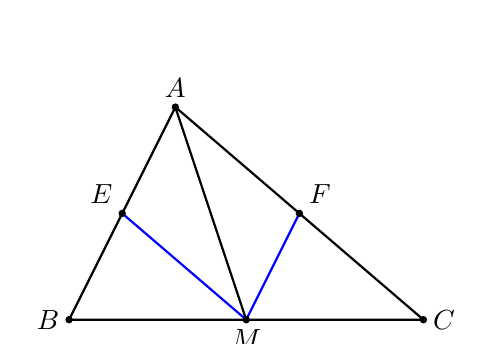
\begin{tikzpicture}[scale=0.9, >=stealth]
  \coordinate (A) at (1.5,3);
  \coordinate (B) at (0,0);
  \coordinate (C) at (5,0);
  \coordinate (M) at ($(B)!0.5!(C)$);
  \coordinate (E) at ($(A)!0.5!(B)$);
  \coordinate (F) at ($(A)!0.5!(C)$);
  \draw[thick] (A)--(B)--(C)--cycle;
  \draw[thick] (A)--(M);
  \draw[thick, blue] (M)--(E);
  \draw[thick, blue] (M)--(F);
  \fill (A) circle (1.5pt) node[above] {$A$};
  \fill (B) circle (1.5pt) node[left] {$B$};
  \fill (C) circle (1.5pt) node[right] {$C$};
  \fill (M) circle (1.5pt) node[below] {$M$};
  \fill (E) circle (1.5pt) node[above left] {$E$};
  \fill (F) circle (1.5pt) node[above right] {$F$};
\end{tikzpicture}
\end{center}
\begin{enumerate}[label=\textbf{\alph*)}, leftmargin=0.8cm, itemsep=0pt, topsep=1pt]
\item (0,4 điểm) Chứng minh tứ giác $AEMF$ là hình bình hành.
\item (0,35 điểm) Nếu $\widehat{BAC} = 90^\circ$, chứng minh tứ giác $AEMF$ là hình chữ nhật. Từ đó suy ra $EF = \dfrac{1}{2}BC$.
\end{enumerate}
\loigiai{
\textbf{a)} \textit (0,4 điểm): Ta có $ME \parallel AC$ nên $ME \parallel AF$ (do $F \in AC$), và $MF \parallel AB$ nên $MF \parallel AE$ (do $E \in AB$). Tứ giác $AEMF$ có các cặp cạnh đối song song nên là hình bình hành.

\textbf{b)} \textit (0,35 điểm): Hình bình hành $AEMF$ có một góc vuông ($\widehat{EAF} = \widehat{BAC} = 90^\circ$) nên là hình chữ nhật. Do đó hai đường chéo bằng nhau: $EF = AM$. Trong tam giác vuông $ABC$ vuông tại $A$, trung tuyến $AM = \dfrac{1}{2}BC$, suy ra $EF = \dfrac{1}{2}BC$.


}
\end{ex}
\vspace{0.5mm}

\begin{ex} (0,5 điểm)
Chứng minh rằng giá trị biểu thức sau không phụ thuộc vào giá trị của biến $x$:
$$A = (x + 2)^3 - (x - 2)^3 - 12(x + 1)(x - 1)$$
\begin{enumerate}[label=\textbf{\alph*)}, leftmargin=0.8cm, itemsep=0pt, topsep=1pt]
\item (0,5 điểm) Chứng minh giá trị của $A$ không phụ thuộc vào $x$.
\end{enumerate}
\loigiai{
\textbf{a)} \textit (0,5 điểm): Khai triển biểu thức $A$:

$A = (x^3 + 6x^2 + 12x + 8) - (x^3 - 6x^2 + 12x - 8) - 12(x^2 - 1)$

$= x^3 + 6x^2 + 12x + 8 - x^3 + 6x^2 - 12x + 8 - 12x^2 + 12$

$= (x^3 - x^3) + (6x^2 + 6x^2 - 12x^2) + (12x - 12x) + (8 + 8 + 12) = 28$.

Vì $A = 28$ là một hằng số nên giá trị của biểu thức $A$ không phụ thuộc vào giá trị của biến $x$.


}
\end{ex}
\vspace{0.5mm}


\enlargethispage{1.5cm}
\begin{center}
\rule{4cm}{0.4pt}\\
\textit{--- HẾT ---}
\end{center}
\end{document}
